\chapter{MHD waves and spectroscopy} \label{ch: spectroscopy}

\graphicspath{{02-MHD_spectroscopy/figures/}}

\begin{chapterquote}[Eugene Parker][][]
  I'm proud of the fact that I thought of the solar wind. It was an exercise in pursuing curiosity, which is the main motivation for studying physics from a personal standpoint.
\end{chapterquote}

This Chapter provides an overview of the main principles of MHD spectroscopy and how one usually goes about detailing all waves and instabilities of a given physical equilibrium. Doing so can either be straightforward and yield relatively simple results, or can be quite complicated to the point where solutions show so many detailed features and intricacies that it is difficult to see the forest for the trees. Due to this inherent range in complexity of the problem at hand we adopt a step-by-step approach. Focusing on uniform equilibria at first, we look into simple waves and instabilities present in these plasmas and pay special attention to how the spectrum changes when more physics are included. In this Chapter we will limit ourselves to non-adiabatic effects: heating, cooling and thermal conduction.

This will already provide us with a myriad of information regarding the underlying physics at play in simple configurations, though eventually we want to move on to more realistic equilibria by introducing non-uniformity in the background. At that point we will hit the limit of what can be solved analytically, and the discussion in this chapter will shift to a more qualitative approach. This will get picked up again in later Chapters, where we will go more in-depth on how to tackle this particular problem and take a closer look at all the interesting features that emerge when solving it.

\section{Introduction}
Magnetohydrodynamics (MHD) is the cornerstone of plasma physics, and in an ideal setting describes the behaviour of a perfectly conducting fluid when it interacts with a magnetic field. In essence, MHD combines the Euler equations of gas dynamics with Maxwell's equations to describe the evolution of a magnetised plasma on macroscopic scales. This is the direct opposite of \emph{kinetic theory} (basically the other cornerstone of plasma physics), which describes plasmas using a collection of microscopic particles.

We will not go in-depth as to which theory is better suited for one particular problem or under which conditions they are valid approximations. Generally speaking if one is investigating very small spatial or temporal scales then kinetic theory is the best option. On the other hand, for ``larger'' applications in which one assumes that the collisions between individual particles happen so frequently that the plasma can be treated as a single continuous fluid then MHD is the way to go. This also means that effects due to collective particle phase-space are ignored however, implying that kinetic theory is more complete as a physical model, at the expense of increased complexity. Throughout this thesis we will always assume that plasma is a single continuous fluid, and we stick with the MHD representation.

One beautiful feature of the MHD equations is that they are \emph{scale-independent}. The equations themselves are made dimensionless by choosing (generally speaking) reference values for the typical length scale, magnetic field strength and plasma density, as for example explained in \citet[Chapter 4]{book_MHD}. Depending on the problem at hand different reference values can be chosen to describe the situation, which in turn implies that MHD can describe plasmas in astrophysical settings (accretion disks, jets around black holes, stellar atmospheres, etc.) as well as laboratory settings, all using the same set of equations!
\emph{Throughout this thesis we will always work with normalised quantities, unless explicitly specified otherwise.}


\section{Magnetohydrodynamics}
\subsection{The ``simple'' MHD equations}
We first start with ``simple'' MHD, that is, constraining ourselves to the ideal equations. The word ``simple'' is placed between quotation marks here, as the ideal MHD equations are rather straightforward compared to their counterparts in which various non-ideal physical effects have been added. However, from a mathematical point of view even these relatively simple equations still describe a system of eight hyperbolic partial differential equations, which are \emph{not at all} easy to solve. For that we have to rely on numerical methods and dedicated codes, which are whole topics in itself. As the explicit derivation of these equations is standard material in any textbook on plasma physics, for example \citet{book_priest, book_davidson} or \citet{book_choudhuri}, with my favourite being \citet{book_MHD}, we will simply give their final (ideal) form below.

\begin{gather}
  \frac{\partial \rho}{\partial t} = -\nabla \cdot (\rho \bv), \label{eq: ideal_continuity} \\
  \rho \frac{\partial \bv}{\partial t} =
    -\nabla p
    - \rho \bv \cdot \nabla \bv
    + (\nabla \times \bb) \times \bb, \label{eq: ideal_momentum}\\
  \rho \frac{\partial T}{\partial t} =
    -\rho \bv \cdot \nabla T
    -\gmone p \nabla \cdot \bv, \label{eq: ideal_energy} \\
  \frac{\partial \bb}{\partial t} = \nabla \times (\bv \times \bb), \label{eq: ideal_induction}
\end{gather}
consisting of the continuity equation \eqref{eq: ideal_continuity}, momentum equation \eqref{eq: ideal_momentum}, energy equation \eqref{eq: ideal_energy} and induction equation \eqref{eq: ideal_induction}. The quantities $\rho$, $\bv$, $p$, $\bb$ and $T$ denote the plasma density, velocity field, pressure, magnetic field and temperature, respectively. The ratio of specific heats is denoted by $\gamma$ and is taken to be equal to $5/3$. The system is constrained by the divergence-free condition on the magnetic field $\nabla \cdot \bb = 0$, ensuring no magnetic monopoles, and the (normalised) ideal gas law $p = \rho T$. In three dimensions this results in eight equations and eight unknown variables $(\rho, \bv, T, \bb)$. Note that the above equations are already in normalised form. The normalisation process itself is quite straightforward: reference values $\{l_0, B_0, \rho_0\}$ are chosen for the length scale, magnetic field, and density, respectively. The reference velocity then follows from the Alfv\'en speed $v_0 \equiv B_0 / \sqrt{\mu_0 \rho_0}$, which in turn constrains the reference time as $t_0 \equiv l_0 / v_0$. All that is left is normalising the differential operators $\bar{\nabla} \equiv l_0 \nabla$ and $\partial/\partial \bar{t} \equiv t_0 \partial / \partial t$; along with the actual variables $\bar{\rho} \equiv \rho / \rho_0$, $\bar{\bb} \equiv \bb / B_0$, $\bar{\bv} \equiv \bv / v_0$, and so on. Applying these transformations keeps the original set of equations unchanged, except that all variables and operators are now equipped with a bar and the quantity $\mu_0$ has vanished. In the above Equations \eqref{eq: ideal_continuity} -- \eqref{eq: ideal_induction} these bars have been dropped since there is no confusion possible.

\subsection{The non-adiabatic MHD equations}
In the previous Subsection we discussed ideal, adiabatic MHD, meaning that no energy is gained or lost by the system and any change in internal energy is due to work. One can now wonder how everything is affected when this is not the case, that is, energy is gained by the system (though heating, for example), at the same time lost through radiation and on top of that there is internal energy transfer through the process of thermal conduction. When these effects are included in our representation we are talking about the \emph{non-adiabatic MHD equations}.

Mathematically the heating and cooling terms are represented by a quantity known as the \emph{heat-loss function} $\HLF$, defined as energy losses minus energy gains
\begin{equation} \label{eq: cooling_simple}
  \HLF(\rho, T) = \rho \HLFcool - \HLFheat,
\end{equation}
which is generally dependent on density and temperature. In this representation the heating function $\HLFheat$ is assumed to be constant in time. The quantity $\HLFcool$ is a tabulated set of temperature-dependent values resulting from detailed atomic and molecular calculations, to which we hereafter refer to as the ``cooling curve''.

For magnetised plasmas heat transfer through thermal conduction has a preferred direction, in this case the effect is a few orders of magnitude stronger along the magnetic field lines than across them \citep{book_spitzer}. To model this anisotropy we make use of the thermal conductivity tensor $\bkappa$, given by
\begin{equation} \label{eq: conduction}
  \bkappa = \kappapara\unit{B}\unit{B} + \kappaperp\left(\idmat - \unit{B}\unit{B}\right).
\end{equation}
Here $\idmat$ is the identity matrix and $\unit{B} = \bb/B$ is a unit vector along the magnetic field. The quantities $\kappapara$ and $\kappaperp$ denote the thermal conduction coefficients parallel and perpendicular to the magnetic field lines and are taken equal to the Spitzer conductivity \citep{book_priest}
\begin{equation} \label{eq: thermal_coeffs}
  \begin{gathered}
    \kappapara \approx 8 \times 10^{-7} T^{5/2}, \\
    \kappaperp \approx 4 \times 10^{-10} n^2 B^{-2} T^{-3} \kappapara,
  \end{gathered}
\end{equation}
both in units of erg cm$^{-1}$ s$^{-1}$ K$^{-1}$. Here $n$ denotes the number density, given by $n = \rho \massp$ with $\massp$ the proton mass. In the equations that follow these coefficients have been normalised using
$\bar{\kappa}_\parallel \equiv \kappapara / \kappa_0$ and $\bar{\kappa}_\perp \equiv \kappaperp / \kappa_0$, with reference value $\kappa_0 \equiv \rho_0 l_0 v_0^3 / T_0$. From this point onwards we will omit the bars and always reference the normalised quantities, unless explicitly stated otherwise.

Both the cooling and conduction terms are then added to the appropriate MHD equation, such that the adiabatic energy equation \eqref{eq: ideal_energy} transforms into the non-adiabatic energy equation
\begin{equation} \label{eq: nonad_energy}
  \rho \frac{\partial T}{\partial t} =
    -\rho \bv \cdot \nabla T
    -\gmone p \nabla \cdot \bv
    -\gmone \rho \HLF
    +\gmone \nabla \cdot \left(\bkappa \cdot \nabla T\right).
\end{equation}


Generally speaking, when numerically solving the system of MHD equations one relies on a similar set of steps no matter the approach taken. First a geometry is chosen depending on the problem at hand: a Cartesian (rectangular) box is convenient when describing for example parts of the solar atmosphere, while cylindrical geometries are more useful to describe problems like expanding flux tubes or jets. Next an initial state is chosen at time $t = 0$ fitting the problem, which essentially boils down to choosing initial prescriptions for $(\rho, \bv, T, \bb)$:
\begin{equation}
  \begin{gathered}
    \rho_\text{i}(\bx) \equiv \rho(\bx, t=0), \qquad T_\text{i}(\bx) \equiv T(\bx, t=0), \\
    \bv_\text{i}(\bx) \equiv \bv(\bx, t=0), \qquad \bb_\text{i}(\bx) \equiv \bb(\bx, t=0),
  \end{gathered}
\end{equation}
all depending on the position vector $\bx$. Since we are dealing with partial differential equations, appropriate boundary conditions must be chosen on all sides of the domain under consideration. Once the initial setup is chosen, the set of equations \eqref{eq: ideal_continuity}-\eqref{eq: ideal_induction} is written in conservative form and the domain is discretised using one particular resolution (or more in cases of mesh refinement). Then the iterative process can start: once one's favourite numerical scheme is chosen all fluxes through every cell in the domain are calculated and the system is advanced in time. These two steps are repeated until the simulation ends and/or the system reaches a stationary state.

Naturally, it is clear that higher resolutions result in much finer cells, which in turn may reveal more features. The major downside here is that more cells require more calculations, and in three dimensions the number of calculations required to advance the simulation even a single timestep scales with the third power in resolution. This requirement can be somewhat mitigated by using mesh refinement, i.e. focusing high resolutions on regions of interest in the domain while keeping the other regions at lower resolutions. In most, if not all, of these cases however one usually has to resort to supercomputers in order to run these simulations at resolutions that properly resolve features of interest.



\section{Introduction to MHD spectroscopy}
The main question that spectroscopy tries to answer is ``\emph{How do you know, without explicitly solving the entire set of equations, whether a given dynamical system is stable or not}''? Figure \ref{fig: stability} gives an illustration of the theoretical approach to linear stability analysis. Consider a solid ball at rest at an initial time $t = 0$ on some sort of hill in a gravitational field. If no forces are acting on this ball, then it will remain in this initial position indefinitely. When a small perturbation is applied, i.e. moving the ball slightly away from its equilibrium position, a number of things may happen depending on the shape of the surface the ball is resting on.

In Panel a the ball is clearly laying on top of a hill, and any shift in initial position will cause it to roll downwards under the influence of gravity. This is called an \emph{unstable} configuration: no matter how small the perturbation is, there is no way to restore the initial equilibrium after the perturbation is applied.
In Panel b we have the exact opposite: shift the ball away from its initial location and it will simply roll downwards again, oscillating back and forth around its position at $t = 0$. Assuming there is some friction present between the ball and the surface, it will eventually come to a standstill again after some time $t$ in the same position as it started in. This is called a \emph{stable} configuration, and in this case even relatively large perturbations will have no major effect on the system as a whole.

\begin{figure}[t]
  \centering
  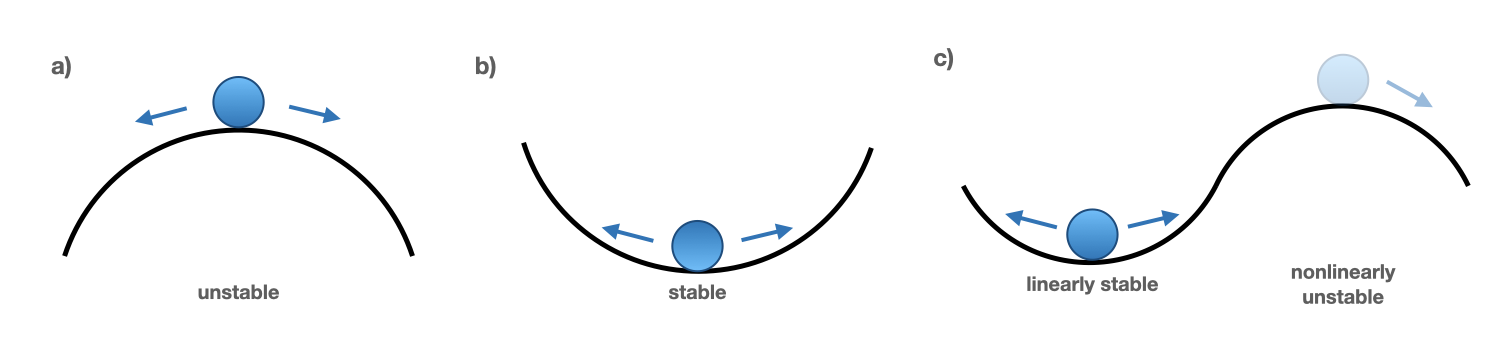
\includegraphics[width=\textwidth]{stability.png}
  \caption{Panel \textbf{a}: Unstable system; Panel \textbf{b}: Stable system; Panel \textbf{c}: Linearly stable, nonlinearly unstable system.}
  \label{fig: stability}
\end{figure}

Panel c on the other hand is much more interesting. Following the same train of thought as for the other two panels, \emph{small} perturbations will return the ball to its equilibrium position. However, if the perturbation is large enough the ball may gain enough energy to reach the peak on the right, roll over, and it will never be able to reach its equilibrium position again. This is called \emph{nonlinear instability}: a system that is stable for small perturbations, but may become unstable for larger perturbations.

Thermal instabilities (TI), the main topic of the next Chapter, can be classified in this latter category. These instabilities are called \emph{thermal} since they originate from the non-adiabatic terms in the energy equation \eqref{eq: nonad_energy}, in particular the radiative cooling terms. A system that is losing energy through radiation and gaining energy through background heating may be stable to small temperature fluctuations, where a restoring force such as magnetic tension/pressure or thermal conduction (which smoothens out variations in temperatures if they are small enough) can counteract the instability and bring the system back in thermal equilibrium. This is the linearly stable regime on the left side of Panel c, Figure \ref{fig: stability}. If the fluctuations are large enough to overcome the restoring forces analogous to the right side of Panel c then a thermal runaway reaction occurs (instability), drastically lowering the temperature. A thorough discussion on the nature of thermal instabilities will be given in the next Chapter.

\subsection{Linearisation of the system}
Now that we have given a simplified example as to get a feel for linear stability analysis, we can start tackling the problem mathematically. Starting with the simplest case, that of a homogeneous background, will already prove quite instructive and will pave the path for more complex treatments later on.

Stability analysis of the MHD equations is done through a process called \emph{linearisation}, which essentially means splitting our equations in an equilibrium part and a dynamical part, where we assume that the latter is a small perturbation (subscript $1$) with respect to the equilibrium state (subscript $0$), such that a quantity $f$ can be written as
\begin{equation} \label{eq: linear_split}
  f(\bx, t) = f_0(\bx, t) + f_1(\bx, t).
\end{equation}
We start by defining the background equilibrium and we hence assume that the dynamics of the system take place around this state. Since we want to start as simple as possible the first assumption we can make is to have a static background, meaning there are no flow effects: $\bv_0 = 0$. The background is also assumed to be constant over time as it is in equilibrium, such that the temporal derivatives evaluate to zero. Furthermore, as mentioned earlier, we first look at a homogeneous background such that it is independent of position and the spatial derivatives become zero as well. The space-time dependence then only enters in the dynamical (perturbed) part of our assumption \eqref{eq: linear_split}. Mathematically this can be written as
\begin{equation} \label{eq: linear_homogeneous}
  \begin{gathered}
    \rho(\bx, t) = \rho_0 + \rho_1(\bx, t), \\
    \bv(\bx, t) = \bv_1(\bx, t), \\
    T(\bx, t) = T_0 + T_1(\bx, t), \\
    \bb(\bx, t) = \bb_0 + \bb_1(\bx, t).
  \end{gathered}
\end{equation}
The next step is plugging these expressions into the system of non-adiabatic MHD equations, and since we are interested in \emph{linear} perturbations we can ignore all higher-order terms $\mathcal{O}(f_1^2(\bx, t))$. Because of our assumptions in \eqref{eq: linear_homogeneous} the divergence-free condition $\nabla \cdot \bb_0 = 0$ is automatically satisfied. We also rewrite the perturbed magnetic field $\bb_1$ in terms of a magnetic vector potential, using $\bb_1 = \nabla \times \ba_1$ such that $\nabla \cdot \bb_1 = \nabla \cdot \left(\nabla \times \ba_1\right) = 0$ is naturally satisfied as the divergence of a curl is always zero by definition.

When the non-adiabatic energy equation \eqref{eq: nonad_energy} is linearised this will contain a term $\rho_1\HLF_0$. Because we linearise around an equilibrium state, we require this state to be in \emph{thermal equilibrium}, implying that all energy gained through heating must be balanced by radiative cooling, resulting in a net difference of zero, hence $\HLF_0$ must be zero. As the heating is assumed to be constant this can be written as
\begin{equation}
  \HLF_0 = \rho_0\Lambda(T_0) - \HLFheat_0 = 0,
\end{equation}
such that the constant heating contribution $\HLFheat_0$ equals the radiative losses $\rho_0\Lambda(T_0)$ at $t = 0$, and the term with $\HLF_0$ drops out of the equations.

The \emph{linearised MHD equations} then read
\begin{gather}
  \frac{\partial \rho_1}{\partial t} = -\rho_0 \nabla \cdot \bv_1, \label{eq: linearised_rho1_homo}\\
  \rho_0 \frac{\partial \bv_1}{\partial t} =
    -\nabla\left(\rho_1 T_0 + \rho_0 T_1\right)
    +\left(\nabla \times \bb_0\right) \times \left(\nabla \times \ba_1\right) \nonumber \\
    +\left[\nabla \times \left(\nabla \times \ba_1\right)\right] \times \bb_0, \\
  \rho_0\frac{\partial T_1}{\partial t} =
    -\rho_0\bv_1 \cdot \nabla T_0
    -\gmone \rho_0 T_0 \nabla \cdot \bv_1
    -\gmone \rho_0 \left(\dHLFT T_1 + \dHLFrho \rho_1\right) \nonumber \\
    +\gmone \nabla \cdot \left(\bkappa_0 \cdot \nabla T_1\right)
    +\gmone \nabla \cdot \left(\bkappa_1 \cdot \nabla T_0\right), \\
  \frac{\partial \ba_1}{\partial t} = \bv_1 \times \bb_0, \label{eq: linearised_A1_homo}
\end{gather}
where the background dimensionless pressure is rewritten as $\rho_0 T_0$ and the perturbed pressure contribution $p_1$ has been replaced by $\rho_0 T_1 + \rho_1 T_0$ following the linearised ideal gas law. The quantities $\dHLFT$ and $\dHLFrho$ denote the temperature and density derivatives of the heat-loss function, respectively, which can be written as
\begin{equation} \label{eq: dHLF_homogeneous}
  \begin{gathered}
    \dHLFrho = \left.\frac{\partial \HLF}{\partial \rho}\right|_\text{T} = \Lambda(T_0), \\
    \dHLFT = \left.\frac{\partial \HLF}{\partial T}\right|_\rho =
      \rho_0 \left.\frac{d\Lambda(T)}{dT}\right|_{\text{T}_0},
  \end{gathered}
\end{equation}
which both have to be evaluated in the equilibrium quantities $\rho_0$ and $T_0$.

This set of linearised equations is still a system of partial differential equations. However, since the homogeneous equilibrium quantities $(\rho_0, \bv_0, T_0, \bb_0)$ do not depend on time and space we can consider plane-wave perturbations of the form
\begin{equation} \label{eq: plane_wave_homogeneous}
  f_1(\bx, t) = \tilde{f_1}\exp\Bigl(\icomplex\bk \cdot \bx - \icomplex\omega t\Bigr),
\end{equation}
where $\bx = (x, y, z)$ is the (Cartesian) position vector, $\omega$ a complex frequency, $\bk = (k_x, k_y, k_z)$ the wave vector and $\tilde{f_1}$ a (complex) constant denoting the amplitude of the plane wave. We are essentially doing a Fourier analysis in three ``ignorable'' dimensions. The wonderful consequence of doing this is that it transforms the temporal and spatial derivatives of the perturbed variables $f_1(\bx, t)$ into
\begin{equation}
  \frac{\partial}{\partial t} \rightarrow -\icomplex\omega, \qquad\qquad
  \nabla \rightarrow \icomplex\bk,
\end{equation}
which reduces the system of partial differential equations to a system of \emph{algebraic} equations given by
\begin{gather}
  \omega \rho_1 = \rho_0 \bk \cdot \bv_1, \label{eq: homo_continuity_algebraic}\\
  \rho_0\omega \bv_1 = T_0 \bk \rho_1 + \rho_0\bk T_1 - \icomplex[\bk \times (\bk \times \ba_1)]\times\bb_0, \\
  \rho_0\omega T_1 =
    \gmone \rho_0T_0 \bk \cdot \bv_1
    - \icomplex\gmone\rho_0\left(\dHLFT T_1 + \dHLFrho \rho_1\right) \nonumber \\
    - \icomplex\gmone \left(\kappapara \kpara^2 + \kappaperp\kperp^2\right)T_1, \\
  \omega \ba_1 = \icomplex\bv_1 \times \bb_0, \label{eq: homo_induction_algebraic}
\end{gather}
with $\kpara$ and $\kperp$ denoting the wave vector components parallel and perpendicular to the background magnetic field $\bb_0$, respectively. As confusion is not possible the tilde notation used in Equation \eqref{eq: plane_wave_homogeneous} has been omitted.

\subsection{Eigenvalues and stability}
The eight equations given in \eqref{eq: homo_continuity_algebraic}-\eqref{eq: homo_induction_algebraic} form a complete eigenvalue problem, with the eigenvectors containing the variables $\rho_1, \bv_1, T_1$ and $\ba_1$. This can be reduced to a standard complex eigenvalue problem of the form $\amat\statevec = \omega\statevec$, with general wave vectors $\bk = (k_x, k_y, k_z)$ and magnetic field vectors $\bb_0 = (B_{0x}, B_{0y}, B_{0z})$. The state vector $\statevec$ containing the unknown variables is then given by
\begin{equation}
  \statevec = \begin{pmatrix}
    \rho_1 & v_{1x} & v_{1y} & v_{1z} & T_1 & A_{1x} & A_{1y} & A_{1z}
  \end{pmatrix}^T.
\end{equation}
Due to the homogeneous background that was imposed the elements of the matrix $\amat$ are constants, and the eigenfrequency $\omega$ of each respective mode can be obtained by directly solving for the eigenvalues of the corresponding $\amat$-matrix. Generally speaking the eigenvalues are complex, hence every eigenvalue can be written as
\begin{equation}
  \omega \equiv \omega_\text{R} + \icomplex\omega_\text{I},
\end{equation}
where $\omega_\text{R}$ and $\omega_\text{I}$ denote the real and imaginary parts, respectively. Looking back at our plane-wave solutions in Equation \eqref{eq: plane_wave_homogeneous} this implies that the temporal behaviour of all waves scales as
\begin{equation}
  \sim \exp(\omega_\text{I} t)\exp(-\icomplex\omega_\text{R} t).
\end{equation}
From this the physical role of both components becomes clear: for purely real eigenvalues ($\omega_\text{I} = 0$) wave modes will propagate in the direction of $\bk$ and oscillate with a frequency $\omega_\text{R}$, these are stable waves and their amplitude will remain constant over time. The sign of $\omega_\text{R}$ represents forwards ($+$) or backwards ($-$) propagating modes with respect to the direction of $\bx$ and the sign of the $\bk$-component. For non-zero $\omega_\text{I}$ however one can distinguish between four scenarios:
\begin{enumerate}
  \item $\omega_\text{R} = 0$ and $\omega_\text{I} > 0$: \emph{unstable modes}. These are imaginary eigenvalues and represent pure instabilities. In this case, if the background is perturbed this will not result in propagating waves but in an exponential increase in amplitude.
  \item $\omega_\text{R} = 0$ and $\omega_\text{I} < 0$: \emph{damped modes}. These are also imaginary eigenvalues but the opposite of the previous case: amplitudes will decay exponentially over time.
  \item $\omega_\text{R} \neq 0$ and $\omega_\text{I} > 0$: \emph{overstable modes}. These eigenvalues are genuinely complex, with nonzero real and imaginary parts. This represents propagating waves which are unstable due to excessive feedback in the system, resulting in an increase in amplitude over time.
  \item$\omega_\text{R} \neq 0$ and $\omega_\text{I} < 0$: \emph{overdamped modes}. The opposite of the previous case, with again eigenvalues that are genuinely complex. These eigenvalues represent propagating waves with decreasing amplitude, eventually dying out such that the system returns to its equilibrium state.
\end{enumerate}

\begin{figure}[b]
  \centering
  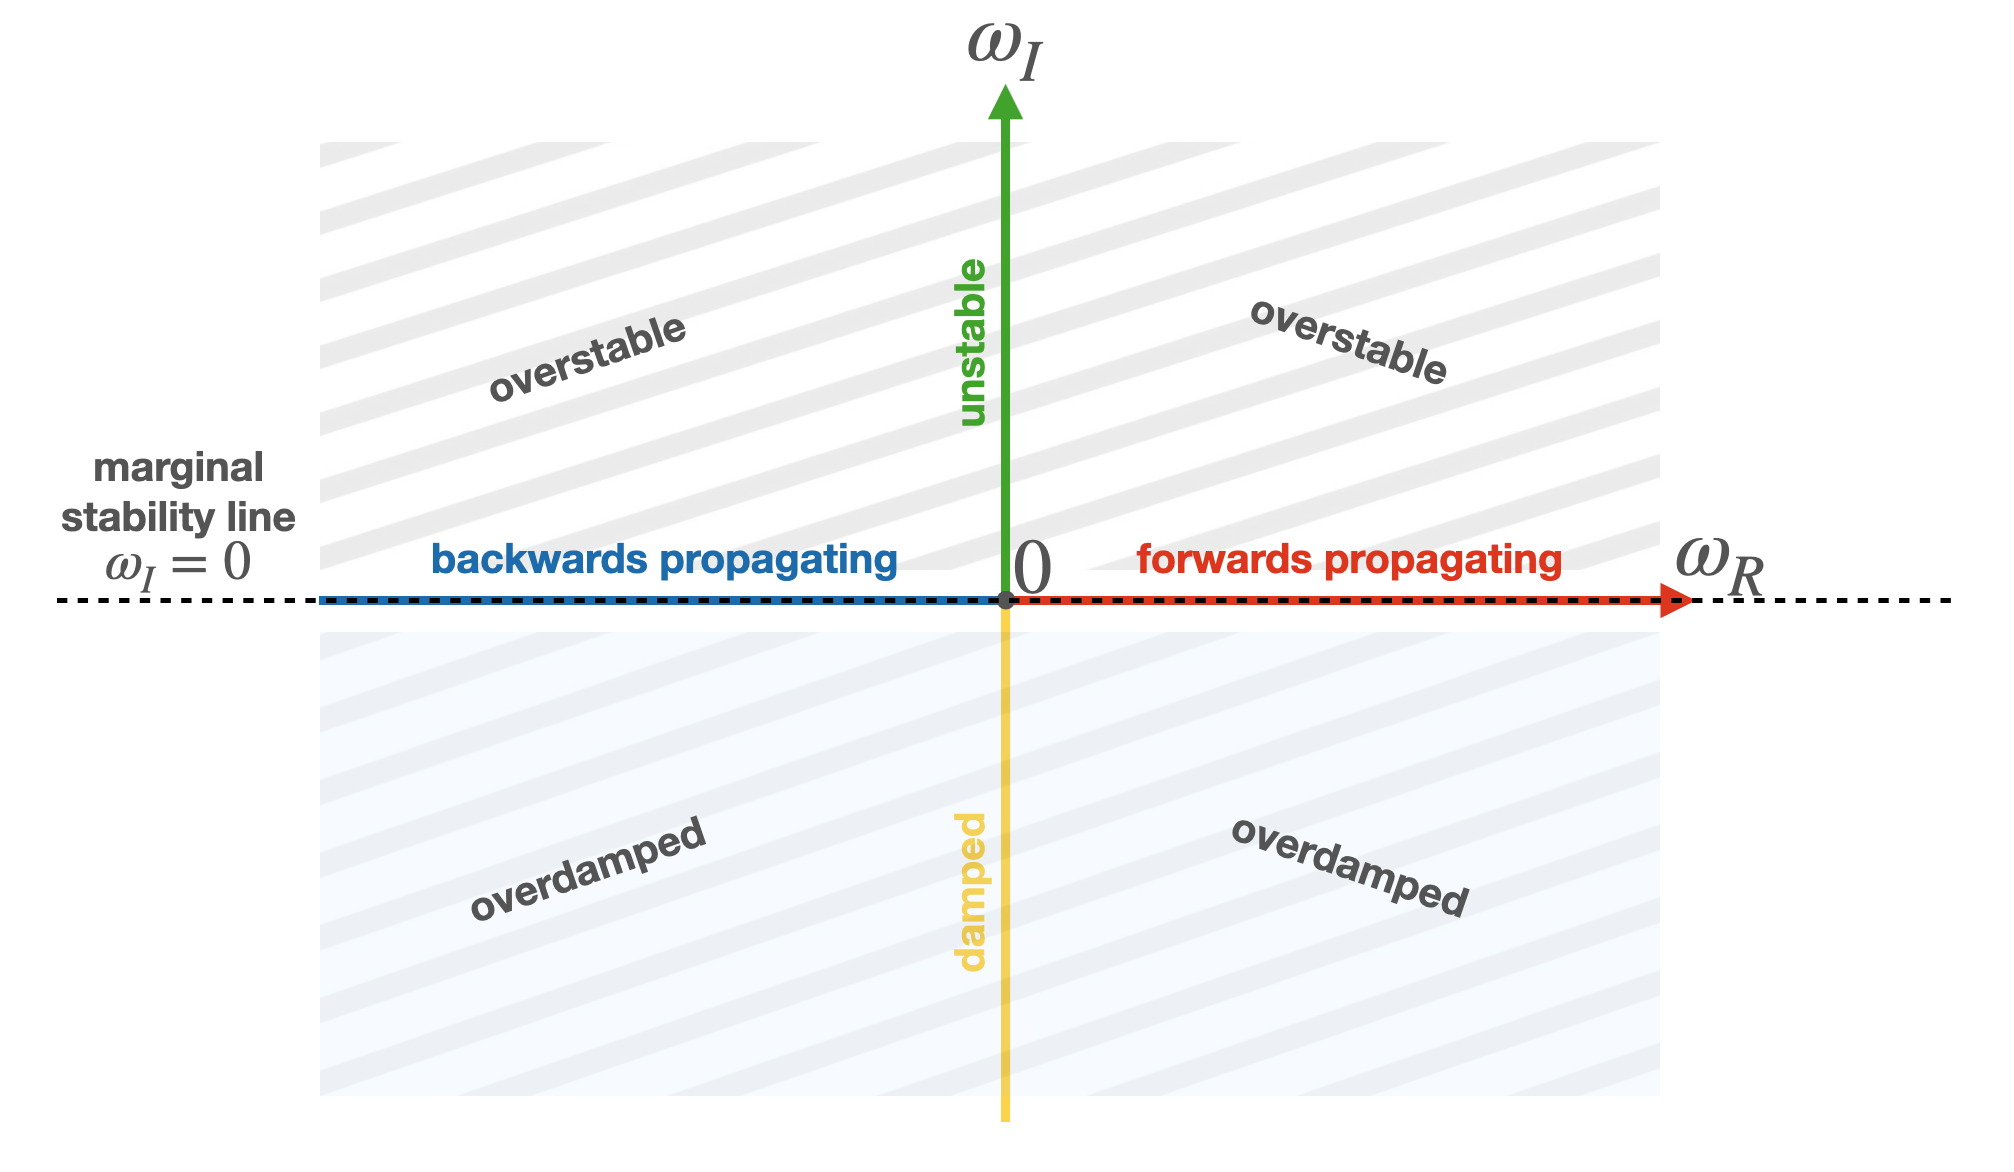
\includegraphics[width=0.9\textwidth]{spectral_plane.png}
  \caption{Graphical representation of various (in)stability regions and their terminology.}
  \label{fig: spectral_plane}
\end{figure}

Figure \ref{fig: spectral_plane} shows a graphical representation of all different cases, where all regions have been annotated in a $\omega_\text{R} - \omega_\text{I}$ 2D-plane. A complex plane like this contains the collection of eigenvalues and is labelled a \emph{spectrum}; we will use similar representations throughout this thesis to visualise eigenvalues. Additionally, in the remainder of this thesis we will not distinguish between damped and overdamped modes, both will simply be referred to as ``damped''.


\subsection{The ideal MHD spectrum}
When solving the eigenvalue system to obtain all eigenvalues some care must be taken, as will become clear in what follows. Since we are dealing with an $8 \times 8$ matrix one would immediately expect that we have eight eigenvalues, and thus eight ``waves'' in our system. In our earlier representation we have chosen a general wave vector and magnetic field vector, but we can always rotate our reference system to choose $\bb_0 = (0, 0, B_0)$ along the $z$-axis and $\bk = (k_\perp, 0, k_\parallel)$ in the $x-z$ plane without losing generality. For the moment we focus on the ideal spectrum, omitting all non-adiabatic effects in the energy equation, such that the $\amat$-matrix in the ideal eigenvalue problem becomes
\begin{equation} \label{eq: ideal_matrix}
  \resizebox{0.89\hsize}{!}{$
    \begin{pmatrix}
      0 & \kperp \rho_0 & 0 & \kpara \rho_0 & 0 & 0 & 0 & 0 \\
      \dfrac{T_0}{\rho_0}\kperp & 0 & 0 & 0 & \kperp & 0 & \dfrac{\icomplex B_0}{\rho_0}k_0^2 & 0 \\
      0 & 0 & 0 & 0 & 0 & -\dfrac{\icomplex B_0}{\rho_0}\kpara^2 & 0 & \dfrac{\icomplex B_0}{\rho_0}\kpara \kperp \\
      \dfrac{T_0}{\rho_0}\kpara & 0 & 0 & 0 & \kpara & 0 & 0 & 0 \\
      0 & \gmone T_0 \kperp & 0 & \gmone T_0 \kpara & 0 & 0 & 0 & 0 \\
      0 & 0 & \icomplex B_0 & 0 & 0 & 0 & 0 & 0 \\
      0 & -\icomplex B_0 & 0 & 0 & 0 & 0 & 0 & 0 \\
      0 & 0 & 0 & 0 & 0 & 0 & 0 & 0
    \end{pmatrix},
  $}
\end{equation}
with $k_0^2 = \kpara^2 + \kperp^2$. This introduces a zero row in the matrix, which essentially originates from the $\nabla \cdot \bb = 0$ constraint which is naturally satisfied in our representation. If we would have kept the magnetic field as-is instead of transforming to a vector potential, this zero row would not have been present. However, in that case we still would have to take the divergence-free constraint into account by eliminating one of the magnetic field variables to obtain a $7 \times 7$ matrix representation. All of this implies that instead of eight solutions to the eigenvalue problem we actually have \emph{seven} solutions and one \emph{spurious} $\omega = 0$ eigenvalue.

In ideal MHD the $\amat$-matrix is Hermitian (i.e. its own conjugate transpose; the matrix operator is self-adjoint), which has interesting consequences for the solutions. From a spectral viewpoint this implies that all eigenvalues either lie \emph{on} the real or imaginary axis, and that there is no possibility to have overdamped or overstable wave modes. Note that this will no longer be the case when we include non-ideal effects, or when we stay ideal but include equilibrium flow.

\paragraph{Entropy solution.}
The first solution is a \emph{genuine} $\omega = 0$ solution (on top of the spurious one), corresponding to a \emph{marginal entropy wave}. It is not of much interest in ideal MHD physically speaking, since it is nothing more than an entropy perturbation. In case of background flow this perturbation will simply be advected along with the velocity field, but will have no effect on the other variables. At this point it is important to stress that this is no longer the case when including non-adiabatic effects: then the entropy solution is shifted from the origin to a purely imaginary solution (corresponding to the thermal instability) which is absolutely physically relevant. The next Chapter will discuss this mode in much more detail.

\paragraph{Alfv\'en waves.}
2 other solutions are the \emph{Alfv\'en waves}, which have their eigenfrequencies given by
\begin{equation} \label{eq: alfvenwaves}
  \omega_\text{a}^2 = \kpara^2 \alfvenspeed^2,
\end{equation}
where $\alfvenspeed^2 = |\bb_0|^2 / \rho_0$ denotes the Alfv\'en speed. These purely transverse anisotropic waves only propagate along the magnetic field lines and owe their origin to restoring forces from magnetic tension effects.

\paragraph{Slow and fast waves}
The final four solutions are called the \emph{slow} and \emph{fast magnetosonic waves}, and their eigenfrequencies are solutions to
\begin{equation} \label{eq: fs_mhd_waves}
  \omega_\text{fs}^2 = \frac{1}{2}k_0^2\Bigl(
    \alfvenspeed^2 + \soundspeed^2 \pm \sqrt{
      \left(\alfvenspeed^2 + \soundspeed^2\right)^2 - 4 \soundspeed^2 \alfvenspeed^2 \cos^2\theta
    }
  \Bigr),
\end{equation}
with $\theta$ denoting the angle between the wave vector $\bk$ and $\bb_0$, the sound speed is given by $\soundspeed^2 = \gamma T_0$. The plus ($+$) and minus ($-$) signs denote the fast and slow MHD waves, respectively. Magnetosonic waves are also anisotropic, although the fast waves are (much) less anisotropic than the slow MHD waves. This follows directly from the definition \eqref{eq: fs_mhd_waves}: if $\cos^2\theta = 0$ (propagation perpendicular to the field lines) then this expression reaches its maximum for the fast wave solution and collapses to zero for the slow wave solution, implying that fast waves propagate faster perpendicular to the magnetic field while slow waves do not propagate in that direction. On the other hand, for $\cos^2\theta = 1$ (parallel propagation) the eigenfrequency for the slow waves reaches its maximum while the fast wave solutions become minimal.

All of these eigenfrequencies follow a strict ordering:
\begin{equation} \label{eq: omega_ordening}
  0 \leq \omega_\text{s}^2 \leq \omega_\text{a}^2 \leq \omega_\text{f}^2 < \infty,
\end{equation}
which is a general property that will be of the utmost importance in spectroscopy, since it determines \emph{the overall structure of an MHD spectrum}. This property will even hold (in one form or another) when we move on to inhomogeneous backgrounds and/or additional physical effects. Figure \ref{fig: adiabatic_spectrum} shows this strict ordering of the eigenfrequencies in the spectral plane, for a general solution of the ideal MHD eigenvalue problem. Note that all eigenfrequencies lie on the real axis, as it should be, owing to the self-adjointness of the matrix operator.

\begin{figure}[t]
  \centering
  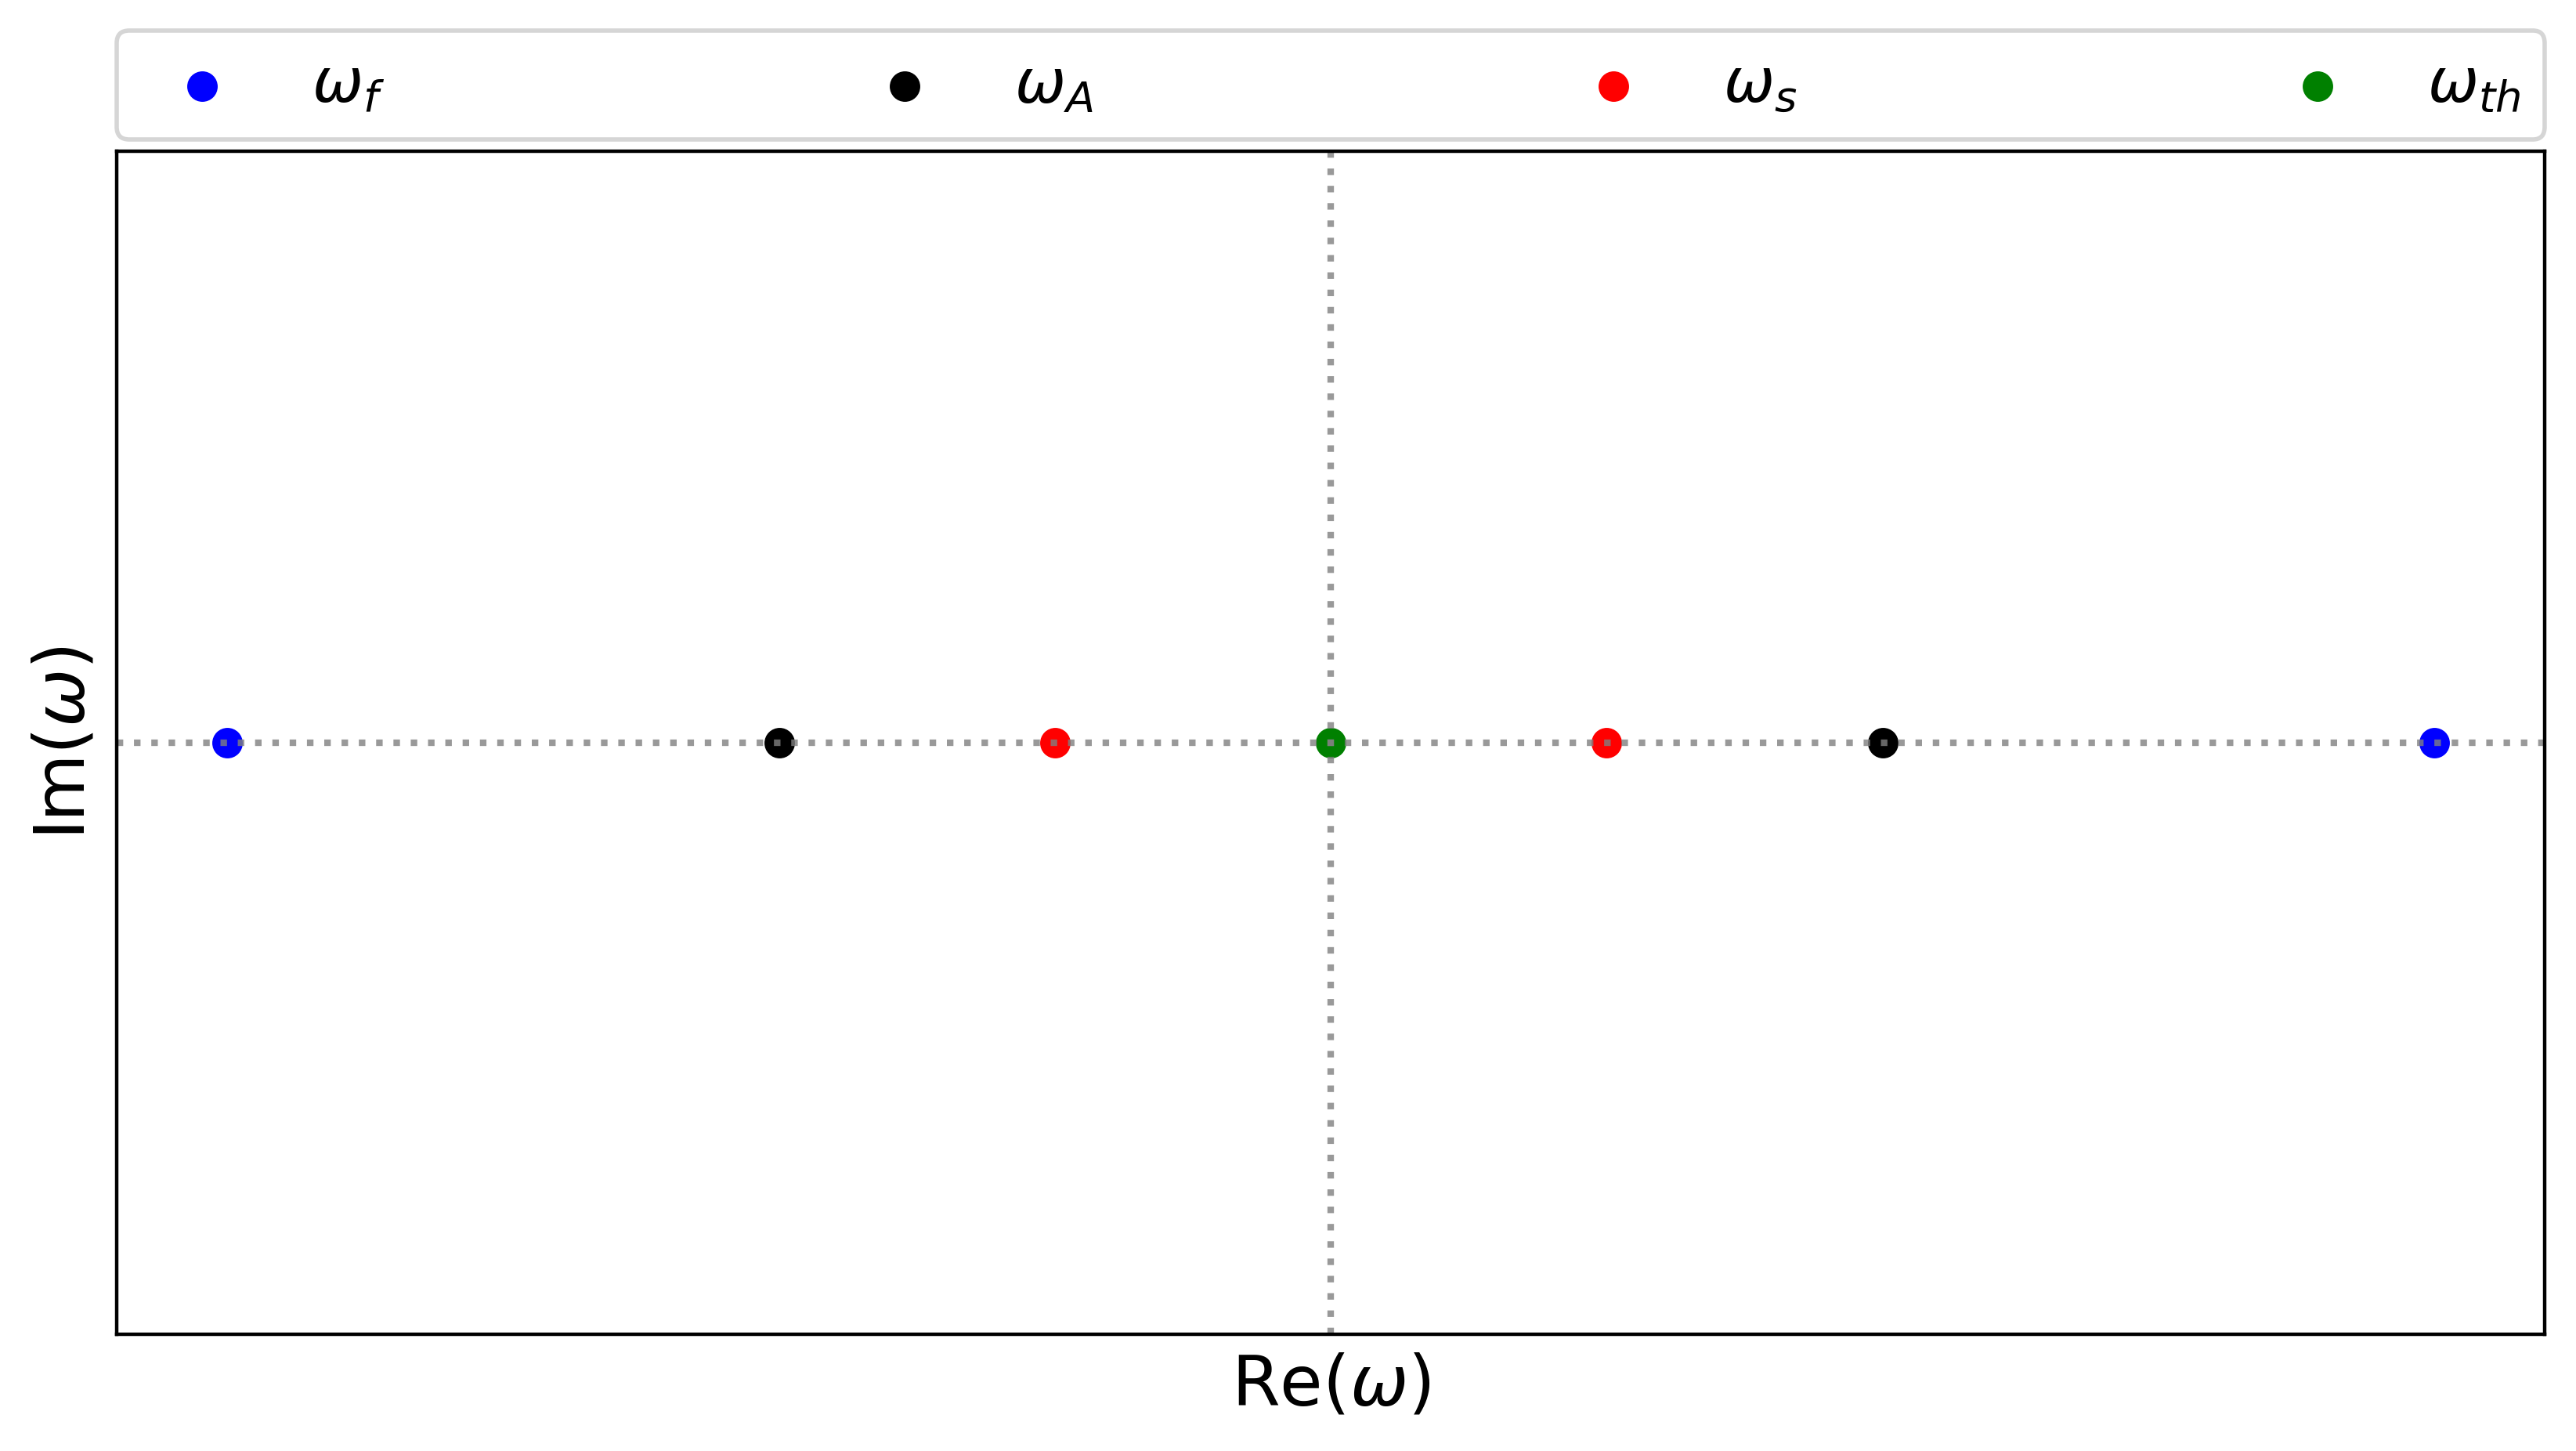
\includegraphics[width=\textwidth]{spectrum_adiabatic.png}
  \caption{
    Visualisation of the ideal MHD spectrum and its seven solutions.
    Blue, black and red dots denote the fast modes, Alfv\'en modes and slow modes, respectively, adhering to the strict ordering in equation \eqref{eq: omega_ordening}. The $\omega = 0$ entropy mode is shown with a green dot, the real and imaginary axes are denoted with dotted lines.
  }
  \label{fig: adiabatic_spectrum}
\end{figure}

\subsection{The non-adiabatic MHD spectrum}
In the previous Subsection we omitted all non-ideal terms in the energy equation \eqref{eq: nonad_energy}, and with the basics in place we can now wonder what will happen to the spectrum when these terms are not omitted. First and foremost, including radiative cooling and/or thermal conduction effects will lift the self-adjointness of the matrix operator, such that genuine complex solutions become possible. The ideal matrix \eqref{eq: ideal_matrix} transforms into its non-adiabatic counterpart
\begin{equation} \label{eq: nonadiabatic_matrix}
  \resizebox{\hsize}{!}{$
    \begin{pmatrix}
      0 & \kperp \rho_0 & 0 & \kpara \rho_0 & 0 & 0 & 0 & 0 \\
      \dfrac{T_0}{\rho_0}\kperp & 0 & 0 & 0 & \kperp & 0 & \dfrac{\icomplex B_0}{\rho_0}k_0^2 & 0 \\
      0 & 0 & 0 & 0 & 0 & -\dfrac{\icomplex B_0}{\rho_0}\kpara^2 & 0 & \dfrac{\icomplex B_0}{\rho_0}\kpara \kperp \\
      \dfrac{T_0}{\rho_0}\kpara & 0 & 0 & 0 & \kpara & 0 & 0 & 0 \\
      -\icomplex\gmone \dHLFrho &
        \gmone T_0 \kperp &
        0 &
        \gmone T_0 \kpara &
        -\dfrac{\icomplex\gmone}{\rho_0}\Bigl(K + \rho_0 \dHLFT\Bigr) &
        0 &
        0 &
        0 \\
      0 & 0 & \icomplex B_0 & 0 & 0 & 0 & 0 & 0 \\
      0 & -\icomplex B_0 & 0 & 0 & 0 & 0 & 0 & 0 \\
      0 & 0 & 0 & 0 & 0 & 0 & 0 & 0
    \end{pmatrix},
  $}
\end{equation}
where we defined $K = \kappapara \kpara^2 + \kappaperp \kperp^2$. Before diving into the modifications this brings to the actual spectrum we first take a look at the $v_{1y}$ component. The third row in this matrix can be written as
\begin{equation}
  \omega v_{1y} = -\frac{\icomplex B_0}{\rho_0}\kpara^2 A_{1x} + \frac{\icomplex B_0}{\rho_0}\kpara\kperp A_{1z}.
\end{equation}
If we combine this with the expressions for the $\omega A_{1x} = \icomplex B_0 v_{1y}$ and $\omega A_{1z} = 0$ components, i.e. the sixth and eight rows of the above matrix, the $v_{1y}$ component can be written as
\begin{equation}
  \omega^2 v_{1y} = \frac{B_0^2}{\rho_0}\kpara^2 v_{1y},
\end{equation}
where we assumed that $\omega \neq 0$ since we are interested in non-zero solutions. This expression is, in fact, equal to the one for the Alfv\'en waves in Equation \eqref{eq: alfvenwaves}, completely decoupled from the other equations. This leads us to an interesting conclusion: \emph{Alfv\'en waves in a homogeneous medium remain unaffected by the inclusion of non-adiabatic effects}; their eigenfrequency will remain exactly the same as for the ideal case.

Figure \ref{fig: nonadiabatic_spectrum} shows a typical spectrum for the non-adiabatic case. Open circles denote the adiabatic solutions, solid dots the non-adiabatic modifications. The arrows indicate the direction of ``movement'' in the spectrum. The thermal mode (green) moves away from the origin and becomes unstable, the slow and fast modes become damped in this case, transforming from purely real to genuinely complex solutions.

Generally speaking the non-adiabatic effects included here have opposite trends with respect to stability, that is, thermal conduction will always try to smoothen out temperature gradients and hence (always) has a stabilising effect, while radiative cooling mostly destabilises. The deciding factor here is the dependence of the heat-loss function on temperature $\dHLFT$. There is a direct link between variations in the cooling curve and thermal mode stability: generally speaking strong variations (larger derivatives) lead to a more unstable thermal mode. Where this behaviour comes from, and which role thermal conduction plays in all this, will be extensively discussed in Chapter \ref{ch: thermal instability}.

\begin{figure}[t]
  \centering
  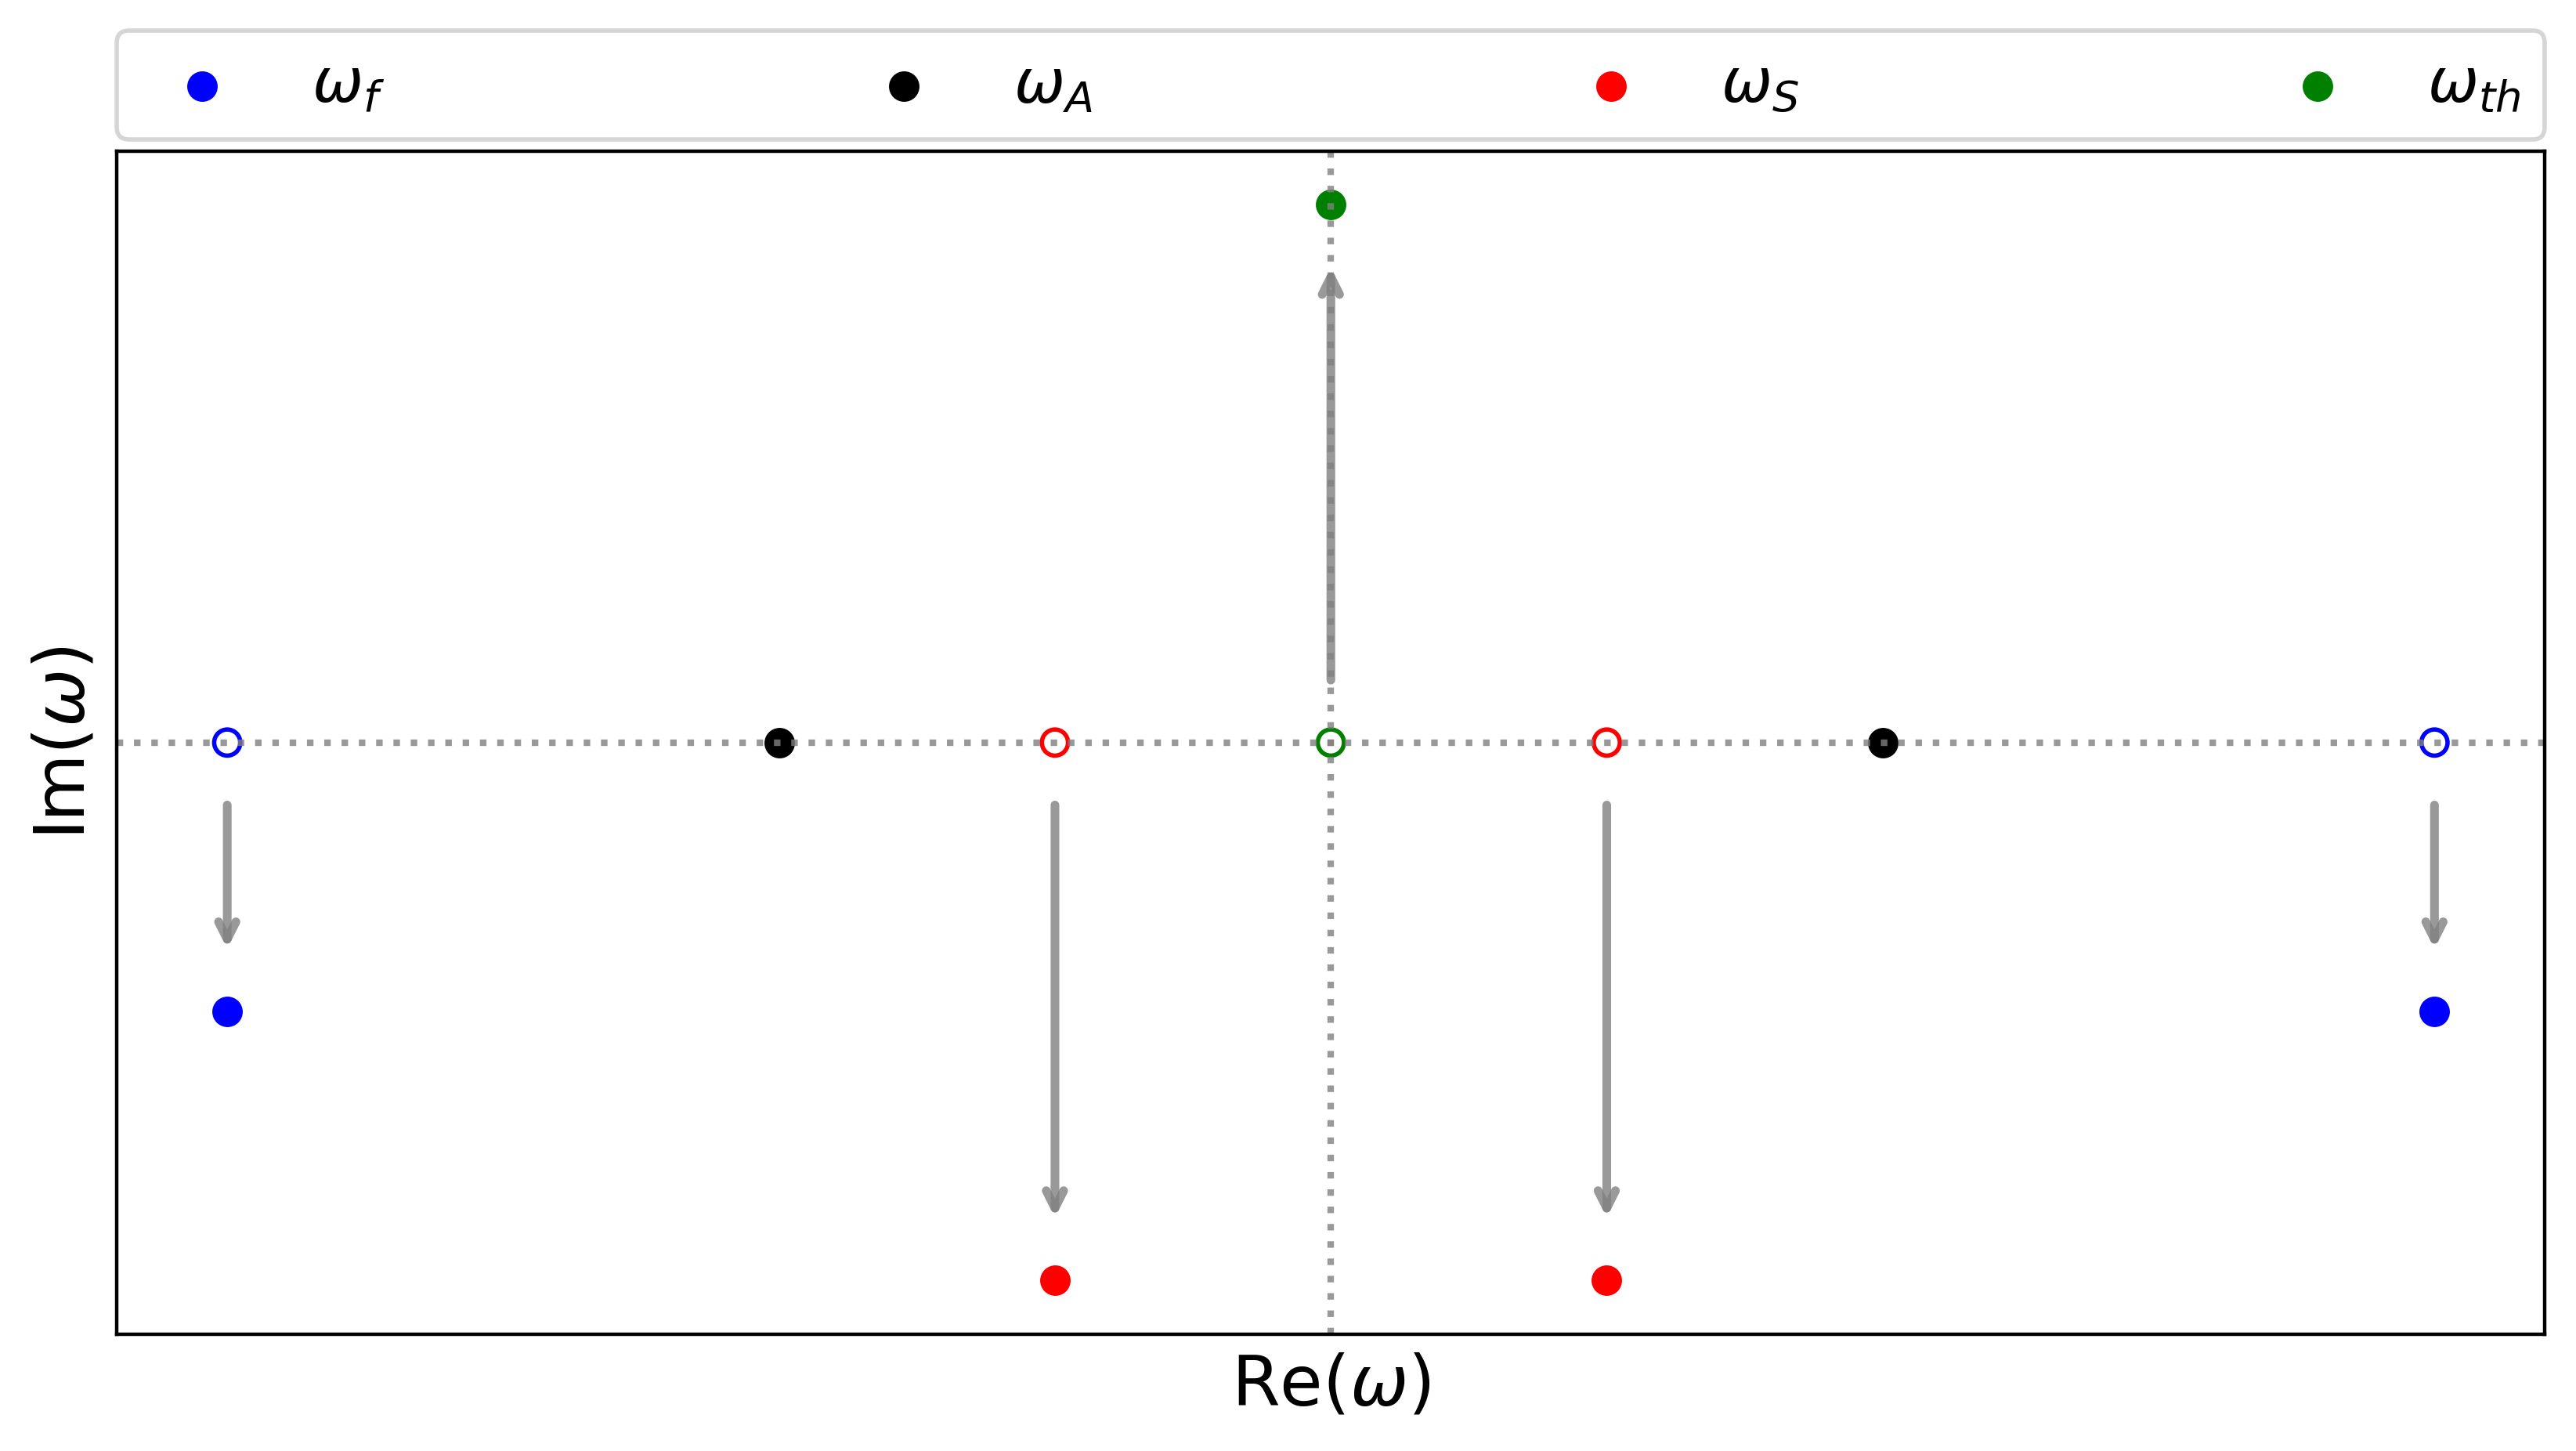
\includegraphics[width=\textwidth]{spectrum_nonadiabatic.png}
  \caption{
    Visualisation of a typical non-adiabatic MHD spectrum; blue, black, red and green dots denote the fast, Alfv\'en, slow and thermal modes, respectively. The empty dots denote the adiabatic solutions, the arrow indicates how these solutions are modified by the additional effects.
  }
  \label{fig: nonadiabatic_spectrum}
\end{figure}


\section{Spectroscopy in non-uniform plasmas}
In all of the above we linearised around a homogeneous background, which allowed us to consider plane-wave perturbations as given in Equation \eqref{eq: plane_wave_homogeneous}. One important remark to be made as well is that the above analysis assumes a medium of infinite extent, i.e. a plasma that is unbounded in all directions.
Nature on the other hand is quite different, since in reality virtually no astrophysical or laboratory plasma configuration is spatially homogeneous, or infinite for that matter. Our initial assumption of uncoupled plane-wave solutions breaks down as soon as we include plasma inhomogeneity, which in turn implies that our operator transformation $\nabla \rightarrow \icomplex\bk$ no longer holds. If we take the direction of inhomogeneity along $x$ then we would have to replace $k_x$ by $\icomplex\partial / \partial x$, and things would get quite complicated real fast. Linearising around a homogeneous background transformed our initial set of partial differential equations to a set of algebraic equations, which could simply be solved by plugging the resulting eigenvalue problem in any modern solver and calculating the eigenvalues. For an inhomogeneous background that depends on $x$ however, the eigenvectors themselves will also depend on $x$, hence all $\nabla$-operators will introduce first (or even second) order derivatives with respect to $x$. This implies that our initial, standard eigenvalue problem $\amat \statevec = \omega \statevec$ will be transformed to a general, complex eigenvalue problem of the form $\amat \statevec = \omega \bmat \statevec$, where the $\amat$ and $\bmat$ matrices \emph{themselves} will contain derivatives of the background quantities, and on top of that the state vector $\statevec$ will contain derivatives of the perturbed quantities as well. At this point most analytical attempts to solve this system will prove impossible and a numerical approach becomes essential.
Before diving into this however, which we will extensively do in Chapter \ref{ch: legolas} and further, we can already familiarise ourselves quite a bit by looking at a relatively simple extension to our homogeneous treatment. This Section builds upon the discussion given in \citet{book_MHD} regarding inhomogeneous plasmas.

\subsection{Spectral symmetry}
Up to now we have neglected to mention a very important property of MHD spectroscopy: that of \emph{spectral symmetry}. This is directly linked to the overall structure of the MHD spectrum, and by extension to the self-adjointness of the matrix operator. These symmetry considerations will remain valid when we later move on to spectroscopy in inhomogeneous plasmas, and have also been partially discussed in \citet{claes2020_legolas}.

We already mentioned a couple of times that the adiabatic linear MHD equations result in a Hermitian eigenvalue problem, hence all eigenfrequencies will be either fully real (stable modes) or fully complex (pure damped or unstable waves) and lie on the real or imaginary axis in the spectral plane. This implies that the full ideal MHD spectrum is \emph{up-down and left-right symmetric}: every mode will have a counterpart mirrored around the corresponding axis, as already seen in Figure \ref{fig: adiabatic_spectrum}. This is directly related to the forward and backwards propagating mode symmetry mentioned earlier, or, equivalently, parity-time symmetry: all these cases are time-reversible.

Including non-ideal effects like radiative cooling and thermal conduction (or e.g. resistivity) lifts the self-adjointness of the eigenvalue problem, allowing the eigenmodes to move away from the axes into the complex plane which will have influence on the symmetry. As long as we are considering static plasmas, that is, no background flow, \emph{left-right symmetry will be preserved}. The inclusion of non-adiabatic effects will however break up-down symmetry as can be seen in Figure \ref{fig: nonadiabatic_spectrum}, but we still have a complementary mode that lies mirrored around the imaginary axis. These spectra correspond to time-irreversible cases.

Finally, including flowing plasmas will introduce a Doppler shift into the spectrum, which in turn is responsible for breaking of left-right symmetry. Ideal, flowing plasmas are in fact governed by a pair of self-adjoint matrix operators \citep{book_MHD}, and every overstable mode has a damped counterpart at the same frequency mirrored around the real axis.

Generally speaking, combining the above statements on spectral symmetry we can summarise as follows:
\begin{itemize}
  \item Static, adiabatic plasmas: \emph{up-down and left-right symmetric}. The eigenvalue problem is Hermitian and all solutions will lie on the real or imaginary axis.
  \item Static, non-ideal plasmas: \emph{left-right symmetric}. The inclusion of non-ideal effects breaks up-down symmetry.
  \item Flowing, adiabatic plasmas: \emph{up-down symmetric}. The Doppler shift introduced by the background flow profile breaks left-right symmetry.
  \item Flowing, non-ideal plasmas: \emph{no symmetry in general}. The combination of flow and non-ideal effects like radiative cooling or resistivity will break left-right and up-down symmetry.
\end{itemize}

From this the wide range in complexity for an MHD spectrum becomes clear: depending on the physical effects taken into account a single spectrum can become extremely complicated. In reality very few astrophysical plasmas can be considered ideal or static, such that in general there will be no spectral symmetry present. In some select cases symmetry can be restored however, even for non-ideal flowing plasmas, by considering a symmetric flow profile in a symmetric domain. This in turn makes the forward and backward modes behave symmetrically, reducing the complexity a bit. This is not always possible however, and generally speaking one will always have to deal with non-symmetric spectra when looking at realistic configurations. In those cases inhomogeneity will also play a major role, which in turn increases the complexity even further due to the presence of the various continua. We will give a general introduction to the MHD continua in Subsection \ref{ss: mhd_continua}.


\subsection{A first approximation to inhomogeneity}
Consider an inhomogeneous medium along $x$ that is bounded between $x = 0$ and $x = L$ but infinite in the $y$ and $z$ directions. As explained in the introductory paragraph we can no longer Fourier analyse along $x$ and a much more intricate treatment is needed. However, we can roughly approximate this medium by a collection of bounded slabs as shown in Figure \ref{fig: bounded_slab} in an effort to understand the general implications that inhomogeneity brings. We can approximately treat the first slab as being bounded between $x = 0$ and $x = a$ and having homogeneous density, temperature and pressure. Due to the bounded nature of this smaller slab the wave number along $x$ will be quantised: $k_x = n\pi / a$ where $n$ is an integer. This in turn introduces a quantisation of the spectrum itself: for every value of $k_x$ we will have a solution to the ideal, homogeneous eigenvalue problem, leading to a discrete spectrum.

\begin{figure}[b]
  \centering
  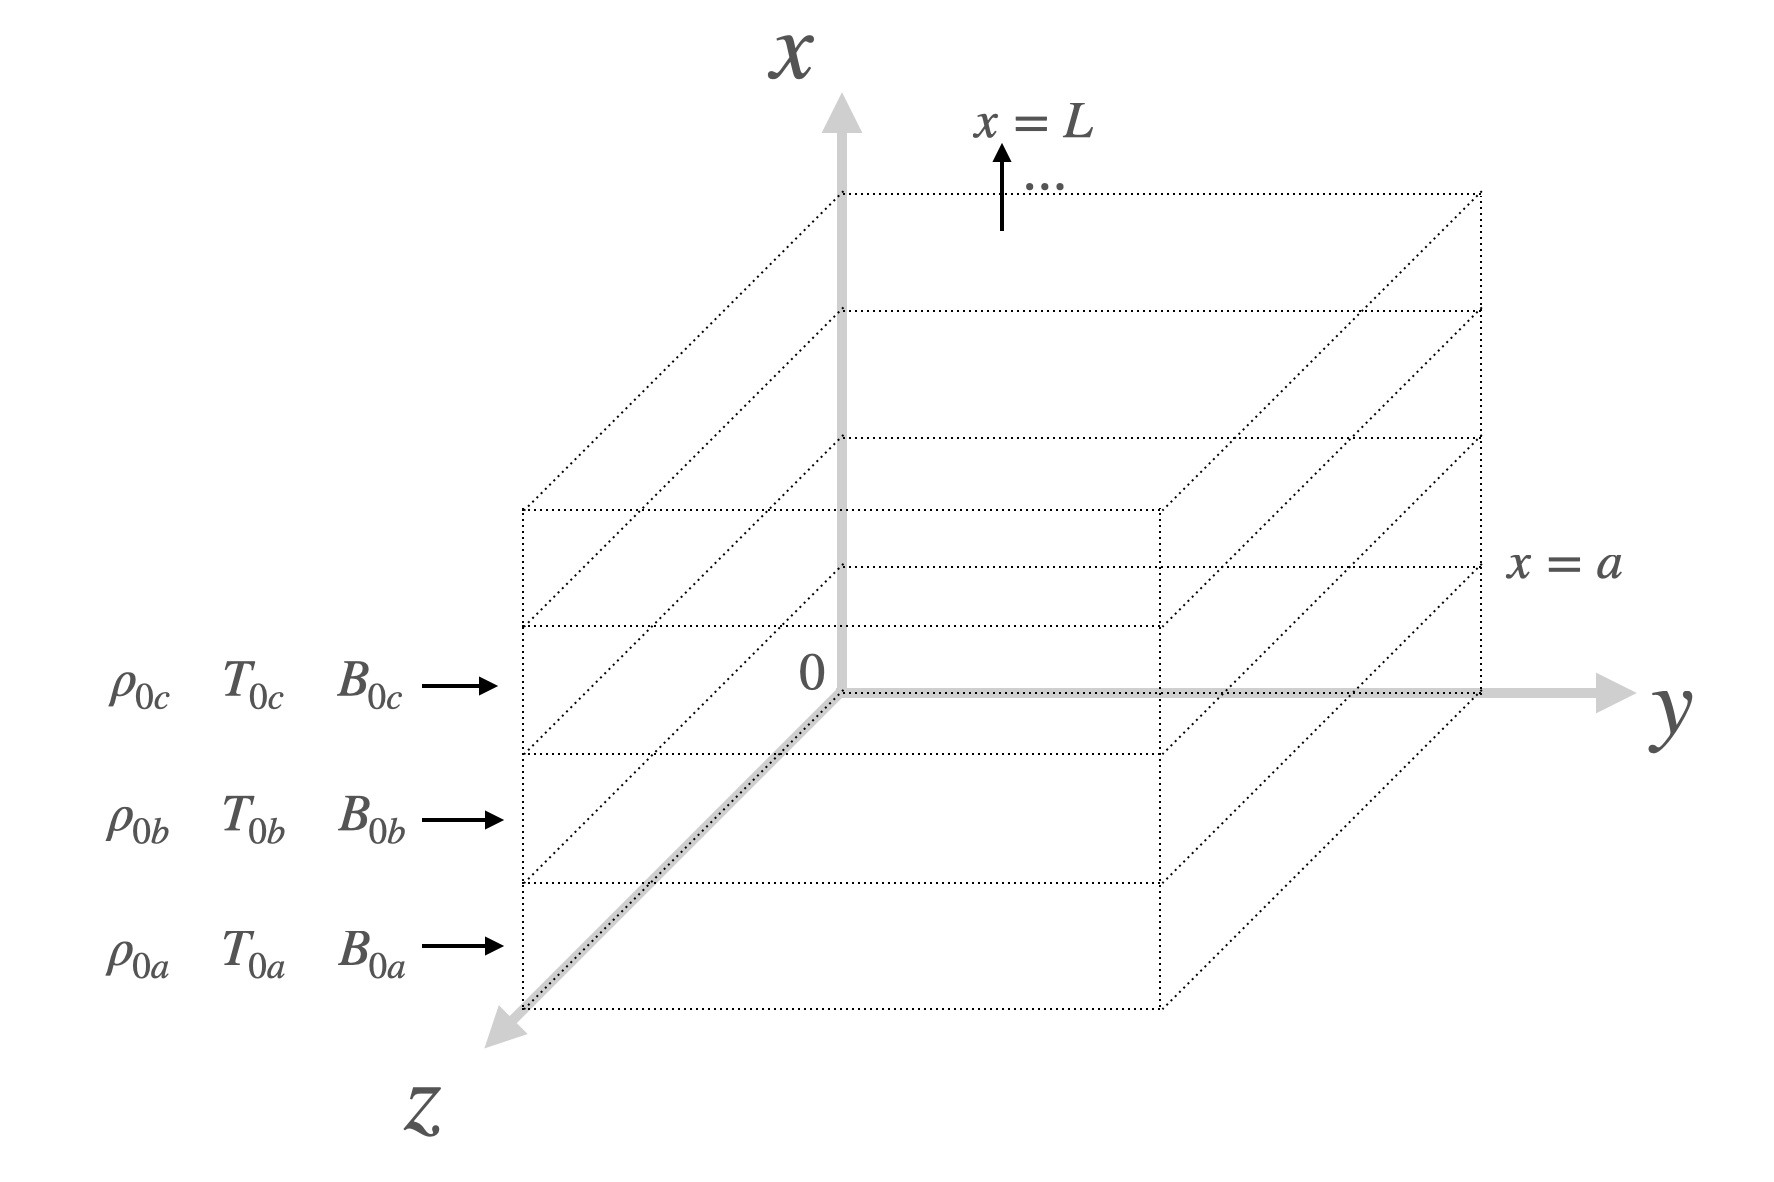
\includegraphics[width=0.7\textwidth]{confined_slab.png}
  \caption{
    An inhomogeneous slab approximated by a collection of homogeneous slabs along $x$, infinite along $y$ and $z$.
  }
  \label{fig: bounded_slab}
\end{figure}

We can understand what this would look like, physically speaking, by turning to the eigenfrequency solutions given in Equations \eqref{eq: alfvenwaves}-\eqref{eq: fs_mhd_waves} while taking the limit of $k_x \rightarrow \infty$. Using the same assumptions as earlier for $\bk$ and $\bb_0$, that is, $\bb_0 = (0, 0, B_0)$ and $\bk = (\kperp, 0, \kpara)$, we get for the Alfv\'en waves
\begin{equation} \label{eq: alfven_accumulation_point}
  \omega_\text{A}^2 = \lim_{\kperp \rightarrow \infty}\omega_\text{a}^2 = \kpara^2\alfvenspeed^2,
\end{equation}
meaning that the Alfv\'en modes are \emph{infinitely degenerate} since they do not depend on $\kperp$. There is hence no difference between $\omega_\text{a}^2$ and $\omega_\text{A}^2$ in this case.

For the slow modes on the other hand we find that
\begin{equation} \label{eq: slow_accumulation_point}
  \omega_\text{S}^2 =
    \lim_{\kperp \rightarrow \infty}\omega_\text{s}^2 =
    \kpara^2 \frac{\alfvenspeed^2 \soundspeed^2}{\alfvenspeed^2 + \soundspeed^2} =
    \frac{\gamma \rho_0 T_0}{\gamma \rho_0 T_0 + B_0^2}\omega_\text{A}^2,
\end{equation}
which, for constant sound- and Alfv\'en speeds (which is the case here as the background is homogeneous), leads to an \emph{accumulation} point in the slow wave sequence. The fast waves have this accumulation point at infinity, since
\begin{equation} \label{eq: fast_accumulation_point}
  \omega_\text{F}^2 = \lim_{\kperp \rightarrow \infty}\omega_\text{f}^2 = \infty.
\end{equation}
Note that we annotated these peculiar frequencies with a capital subscript, as they play a very special role in the eigenspectrum of inhomogeneous plasmas: there the slow accumulation point and degenerate Alfv\'en frequency will get replaced by a continuous range of modes, the slow and Alfv\'en continua, which will be introduced in Subsection \ref{ss: mhd_continua}.

\begin{figure}[t]
  \centering
  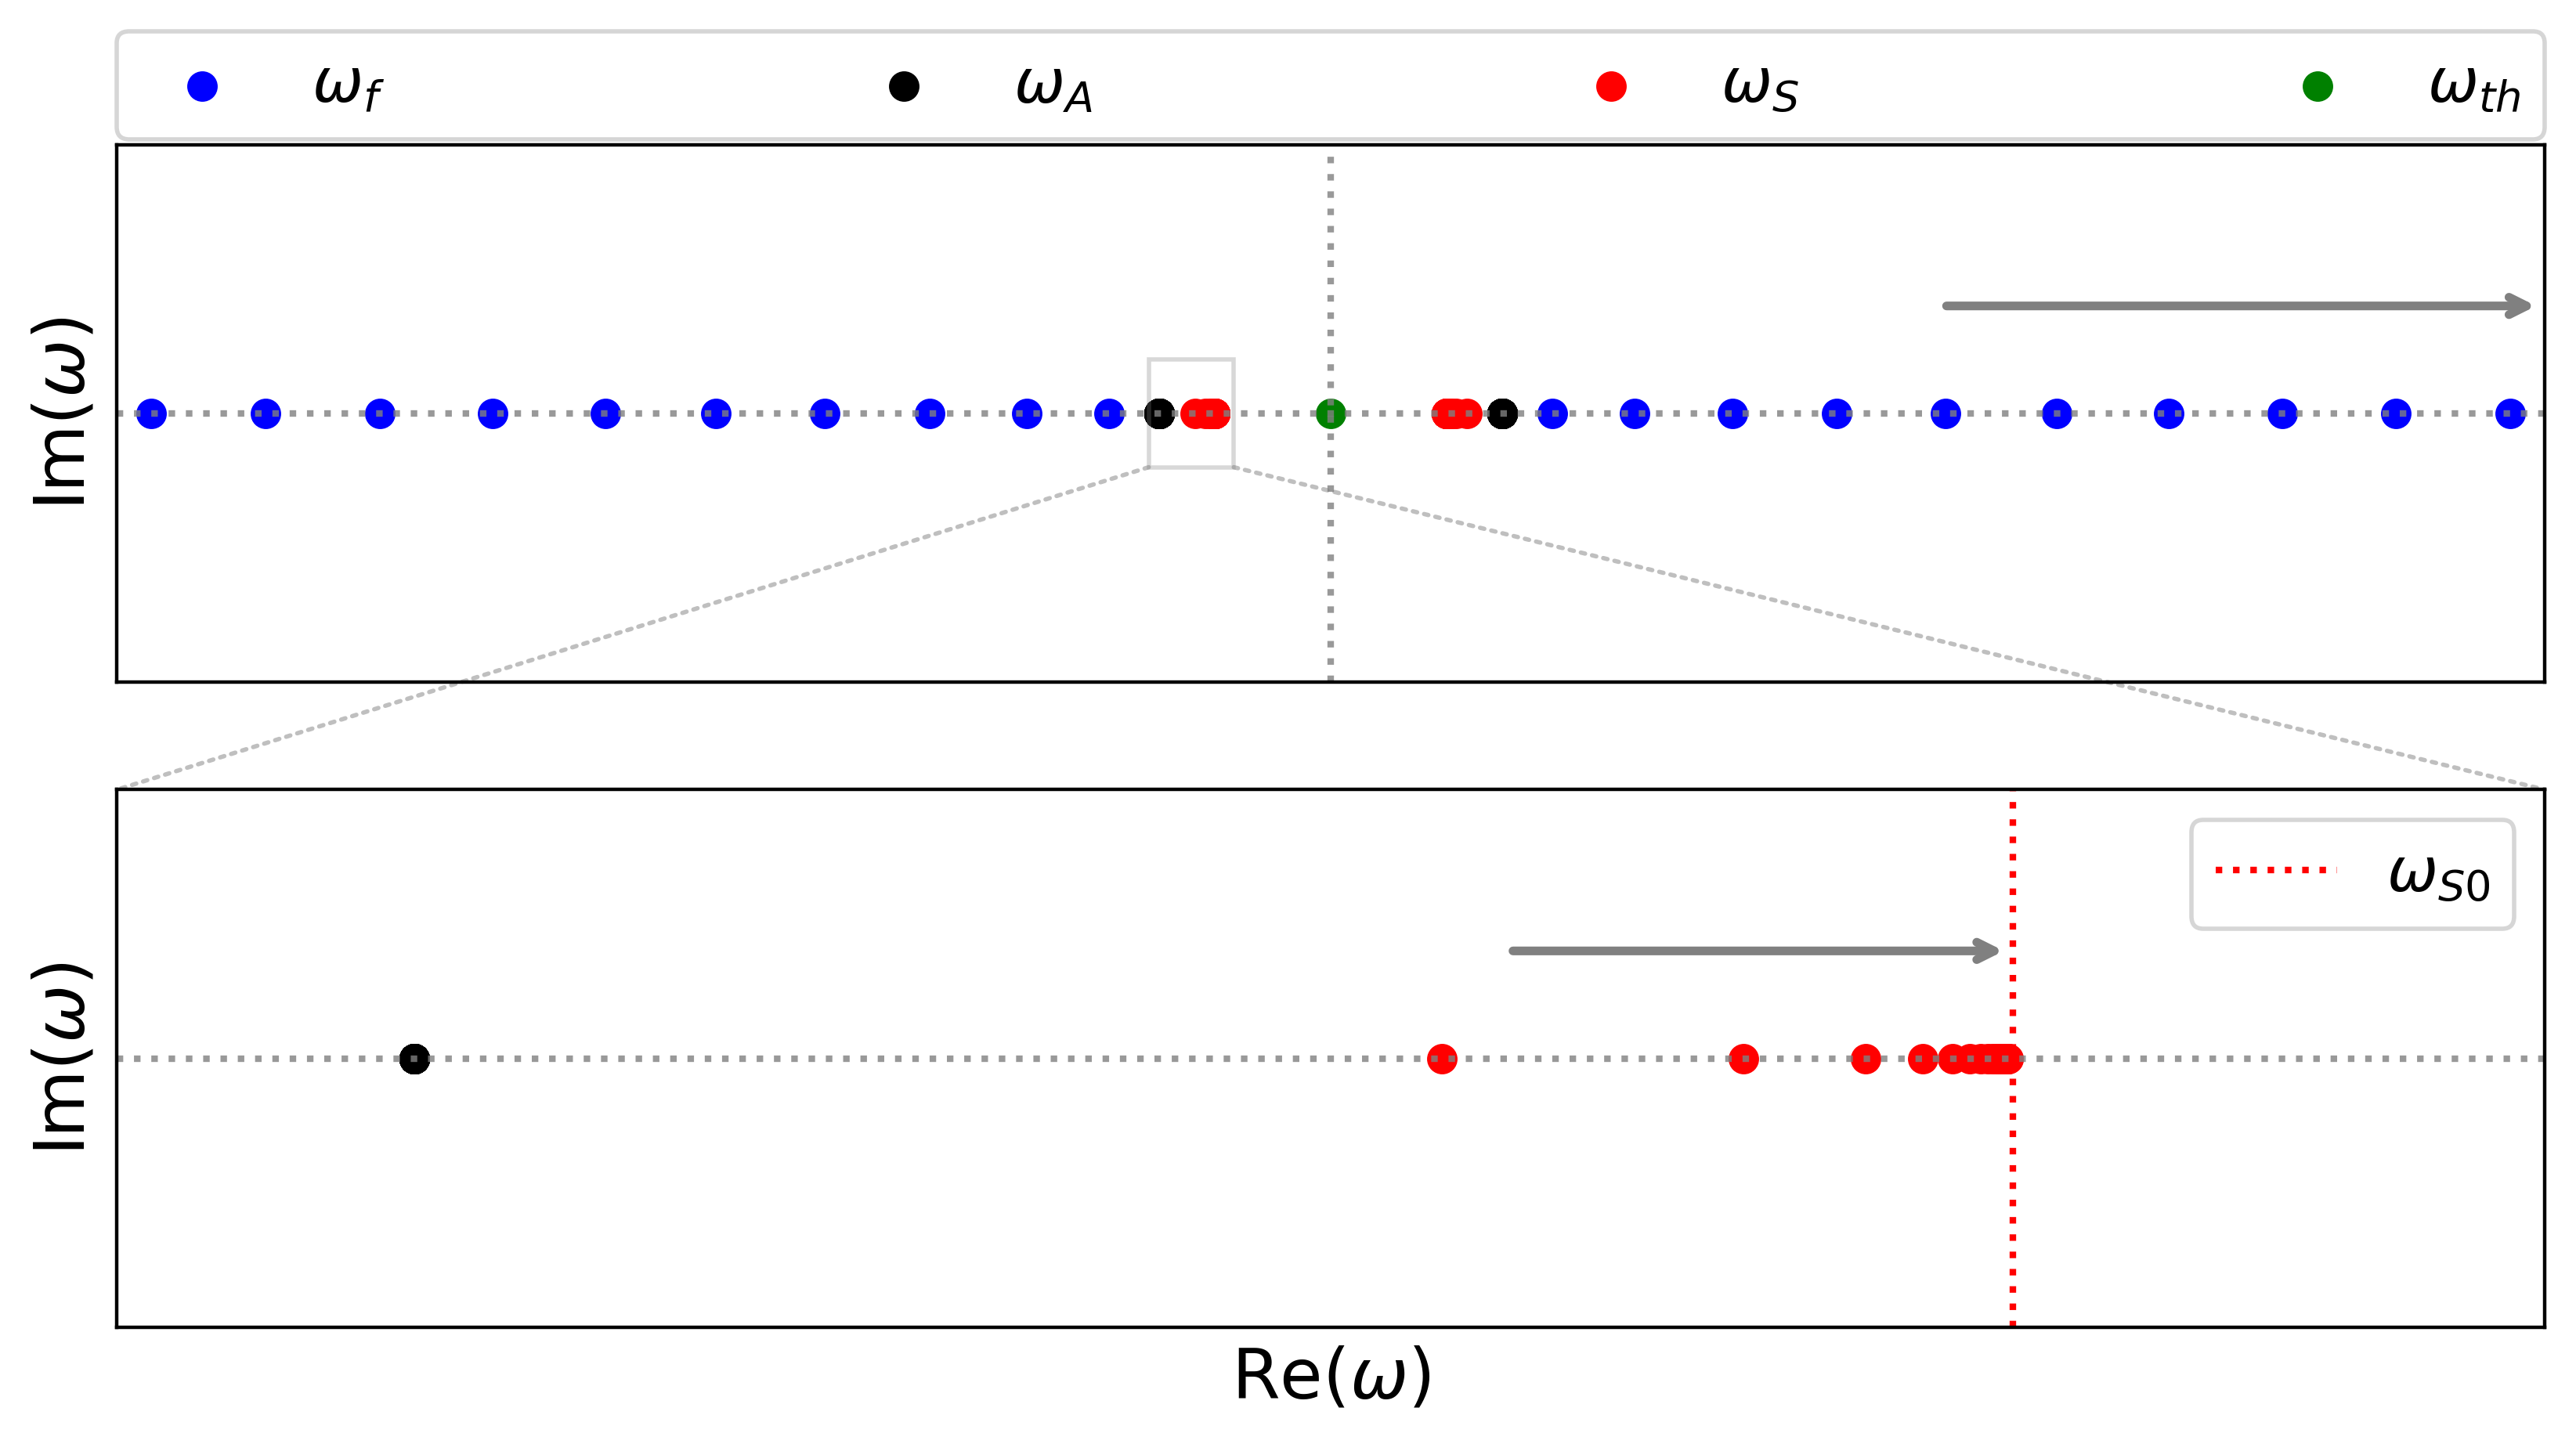
\includegraphics[width=\textwidth]{bounded_ideal_spectrum.png}
  \caption{
    Visualisation of the ideal MHD spectrum for a bounded homogeneous medium. Panel \textbf{a}: overall view of the spectrum, the arrow indicates that the fast modes accumulate at infinity.
    Panel \textbf{b}: zoom of Panel \textbf{a}, clearly showing the degenerate and accumulating behaviour of the Alfv\'en and slow modes, respectively. The slow accumulation point $\omega_\text{S}$ is denoted with a red dotted line, the arrow indicates the direction of increasing $n$.
  }
  \label{fig: bounded_spectrum}
\end{figure}

Figure \ref{fig: bounded_spectrum} shows solutions to the ideal eigenvalue problem, similar to Figure \ref{fig: adiabatic_spectrum}, but for a quantised $\kperp$. Panel a shows an overall view, where the arrow above the fast modes indicates their accumulation point at infinity. Panel b zooms in on Panel a, showing the degenerate behaviour of the Alfv\'en waves and the accumulation sequence of the slow modes. The red dotted line denotes the slow accumulation point $\omega_S$ given by Equation \eqref{eq: slow_accumulation_point}, the arrow indicates the direction of increasing $n$ in the quantisation of the wave number $\kperp$.

\subsection{Introduction to MHD continua} \label{ss: mhd_continua}
\usespublishedwork{
  This Section is partially based on a discussion in the published work ``Magnetohydrodynamic Spectroscopy of a Non-Adiabatic Solar Atmosphere'', 2021, Solar Physics, 296, 9 \citep{claes2021}. N. Claes wrote the manuscript, R. Keppens contributed to the revision of the paper.
}
\subsubsection{Continua in ideal MHD}
To close this Chapter we will briefly touch upon the MHD continua and their (very) important role in the spectral theory of inhomogeneous plasmas. For an inhomogeneous background it is well known that one can reformulate the ideal MHD equations \eqref{eq: ideal_continuity}-\eqref{eq: ideal_induction} into an ordinary differential equation in terms of the $x$-component of the Lagrangian displacement field. It would be rather extensive to do this here, instead we refer to the detailed discussion given in \citet{book_MHD}.

The existence of the slow and Alfv\'en continua correspond to singular points in this ordinary differential equation (ODE), and these continua essentially represent finite ranges of eigenfrequencies with singular, ultra-localized eigenfunctions. They play a key role in processes like phase mixing, resonant absorption or uniturbulence processes. In ideal MHD, the forward and backward slow and Alfv\'en continua are always real (pure waves), and the eigenfrequency ranges are $x$-dependent when the direction of inhomogeneity in the background is taken along $x$.

The slow, Alfv\'en and fast accumulation points discussed in Equations \eqref{eq: alfven_accumulation_point}-\eqref{eq: alfven_accumulation_point} are actually special situations originating from these continua, in which the continua collapse to degenerate single points in homogeneous media. An intuitive way to look at this is to consider the expression for the Alfv\'en accumulation point $\omega_\text{A}^2 = \kpara^2\alfvenspeed^2$, which depends on the Alfv\'en speed and by extension on the density and magnetic field profiles. For an inhomogeneous background these profiles will depend on $x$, hence the Alfv\'en speed will vary over the domain, and thus the continua as well giving rise to a finite range in eigenfrequency. The same reasoning holds for the slow continuum, and since the fast modes have their accumulation point at infinity (such that they don't give rise to singular points in the ODE) we do not have a ``fast continuum''. Additionally, when viewed as a function of $x$, local minima or maxima in the continua may lead to the presence of additional, discrete sequences of modes that cluster towards these accumulation ranges.

\subsubsection{Continua in non-adiabatic MHD}
The inclusion of non-adiabatic effects introduces the thermal continuum, which in static, non-adiabatic settings is just the entropy (thermal) mode. It was shown by \citet{vanderlinden1991} that these continuum modes are introduced by $\kappaperp = 0$, and hence only exist if there is no thermal conduction perpendicular to the magnetic field lines. For nonzero $\kappaperp$ the thermal continuum gets replaced by a quasi-continuum, represented by a dense band of discrete thermal modes. The Alfv\'en continuum remains unmodified when only non-adiabatic effects are included and hence all its continuum solutions will be real, corresponding to locally resonant waves. The slow continuum on the other hand is modified and couples to the thermal continuum, with solutions given by a third-order polynomial in $\omega$
\begin{equation}	\label{eq: slow_thermal_continuum}
  \frac{\rho_0 \left(\soundspeed^2 + \alfvenspeed^2\right)}{\gamma - 1}\icomplex\omega^3
  + \Qai\omega^2
  - \frac{\rho_0 \soundspeed^2\alfvenspeed^2 \kpara^2}{\gamma - 1}\icomplex\omega
  - \Qi\alfvenspeed^2 \kpara^2 = 0,
\end{equation}
with $\isosoundspeed^2 = p_0 / \rho_0$ the isothermal sound speed. The quantities
\begin{equation}
  \begin{gathered}
	  \Qi = \Qifull, \\
    \Qai = \Qaifull,
  \end{gathered}
\end{equation}
are introduced for brevity. Generally speaking, Equation \eqref{eq: slow_thermal_continuum} usually has one purely imaginary solution, corresponding to the thermal continuum $\omega_\text{th}$, and two complex conjugate solutions representing the slow continua $\omega_\text{S}^\pm$. In the ideal case the constant term and the $\omega^2$ term collapse to zero, such that $\omega_\text{th}$ vanishes (reducing to the marginal entropy solution $\omega_\text{th} = 0$). The slow continua reduce to their ideal counterparts $\omega_\text{S}^2 = \kpara^2\soundspeed^2\alfvenspeed^2/(\soundspeed^2 + \alfvenspeed^2)$, which may in turn collapse into points if $\soundspeed$ and $\alfvenspeed$ are both not spatially varying. If the slow continuum vanishes, which is the case if $\bk \cdot \bb_0 = 0$ or if a pressureless background is considered (that is, adopting a zero plasma-$\beta$), the thermal continuum has an analytical solution given by
\begin{equation}
	\omega_\text{th} =
    \frac{\gmone\icomplex}{\soundspeed^2 + \alfvenspeed^2}
    \left[\rho_0\dHLFrho - \dHLFT\left(\isosoundspeed^2 + \alfvenspeed^2\right)\right],
\end{equation}
and hence becomes independent of thermal conduction effects.

\subsubsection{Stability implications of the continua}
It is really important to stress that continuum modes are in fact \emph{actual solutions} to the eigenvalue problem, and hence represent physical modes. Consequently, one can draw the following general conclusions for the stability of a given equilibrium, solely based on the behaviour of its slow and/or thermal continuum regions:

\begin{itemize}
	\item[i)] The continuum regions are partially or fully unstable, that is at least some continuum modes have a positive imaginary part. Since these modes are physical solutions, this means that the medium will be susceptible to instability, either through an unstable slow or thermal mode (or a coalescence of both) depending on which continuum region is unstable. How fast these instabilities form will (usually) depend on the growth rates of the most unstable mode(s), although mode interactions and nonlinear effects can develop quickly.
	\item[ii)] The continuum regions have no internal extrema and are completely stable, that is all modes have a negative or vanishing imaginary part. This corresponds to a stable case, where there is no possibility to trigger instability.
	\item[iii)] The continuum regions have internal extrema. This represents the more general case, in which discrete modes in the vicinity of the continua \textit{may} exist. Here it is possible to have a stable continuum with an unstable discrete mode such that the medium is still unstable.
\end{itemize}

The role of these continua will become clear when we start discussing spectra of inhomogeneous configurations in Chapters \ref{ch: legolas} and \ref{ch: legolas_applications}.

\cleardoublepage
